\documentclass[fullscreen=true, bookmarks=true, hyperref={pdfencoding=unicode}]{beamer}
\usepackage[utf8]{inputenc}                                % Кодировка
\usepackage[english,russian]{babel}                        % Переносы
\usepackage{xcolor}                                        % Работа с цветом
\usepackage{amsmath,amssymb,amsfonts}                      % Символы АМО
\usepackage{graphicx}                                      % Графика
\usepackage[labelsep=period]{caption}                      % Разделитель в подписях к рисункам и таблицам
\usepackage{hhline}                                        % Для верстки линий в таблицах
\usepackage{tikz}                                          % Для простых рисунков в документе
\usepackage{fancybox}                                      % Пакет для отрисовки рамок
\usepackage{verbatim}                                      % Для вставки кода в презентацию
\usepackage{animate}                                       % Для вставки видео в презентацию
\usepackage{xmpmulti}                                      % Для вставки gif в презентацию
\usepackage{multirow}

\usetikzlibrary{arrows, snakes, backgrounds}                 % Для отрисовки стрелок
\usetikzlibrary{positioning, fit, arrows.meta, shapes, calc}
% used to avoid putting the same thing several times...
% Command \empt{var1}{var2}
\newcommand{\empt}[2]{$#1^{\langle #2 \rangle}$}

\graphicspath{{images/}}                                   % Путь до рисунков
\setbeamertemplate{caption}[numbered]                      % Включение нумерации рисунков

\definecolor{links}{HTML}{2A1B81}                          % blue for url links
\hypersetup{colorlinks,linkcolor=,urlcolor=links}          % nothing for others

\usetheme{boxes}
\usecolortheme{crane}

\usepackage{pythonhighlight}

\newtheorem*{question}{Вопрос}

\title{Лекция 3. Рекуррентные нейронные сети}
\author{Александр Юрьевич Авдюшенко}
\institute{МКН СПбГУ}
\date{3 марта 2022}
\titlegraphic{
\includegraphics[keepaspectratio,width=0.5\textwidth]{logo_fmkn.png}}

\begin{document}
%\unitlength=2mm

% выводим заглавие
\begin{frame}
\transdissolve[duration=0.2]
\titlepage
\end{frame}


\begin{frame}
  \frametitle{Пятиминутка}
  \begin{itemize}
    \item Выпишите несколько названий методов оптимизации нейронных сетей
    \item Опишите пару методов регуляризации при обучении нейронных сетей
    \item Нарисуйте (или запишите), как устроен блок skip-connection
  \end{itemize}
\end{frame}


\begin{frame}
  \frametitle{Недостатки сверточных нейронных сетей}
  \framesubtitle{или зачем нужны рекуррентные}
  \begin{itemize}
    \item на входе только вектора фиксированной размерности (например, изображения 28$\times$28)
    \item на выходе тоже размерность фиксирована (например, вероятности 1000 классов)
    \item фиксированное число вычислительных шагов (т.е. архитектура сети)
  \end{itemize}
  \pause
  \href{http://karpathy.github.io/2015/05/21/rnn-effectiveness/}{A. Karpathy. The Unreasonable Effectiveness of Recurrent Neural Networks}
  \begin{center}
    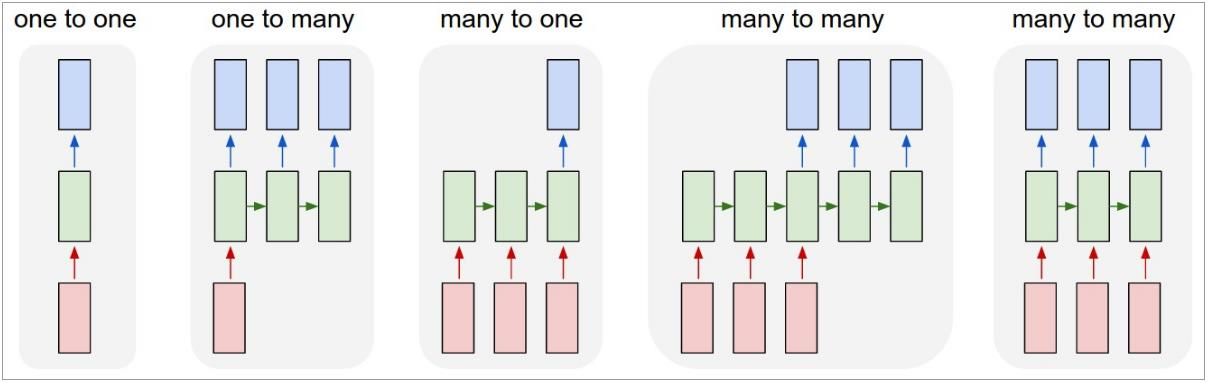
\includegraphics[keepaspectratio,
                     width=0.6\paperwidth]{rnn_architectures.jpg}
  \end{center}
\end{frame}


\begin{frame}
  \frametitle{Архитектуры рекуррентных сетей}
  \begin{tabular}{cc}
    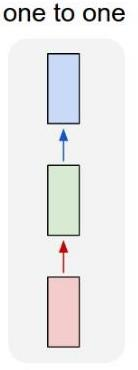
\includegraphics[keepaspectratio,
                     width=0.2\paperwidth]{one-to-one.jpg} &
    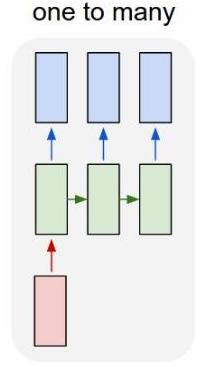
\includegraphics[keepaspectratio,
                     width=0.3\paperwidth]{one-to-many.jpg} \\
    Vanilla Neural Networks & Image Captioning \\
     & image $\to$ (sequence of words)
  \end{tabular}
\end{frame}


\begin{frame}
  \begin{tabular}{cc}
    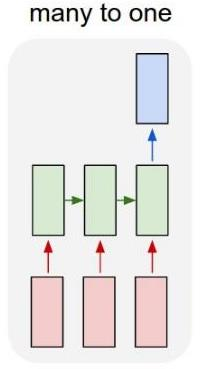
\includegraphics[keepaspectratio,
                     width=0.25\paperwidth]{many-to-one.jpg} &
    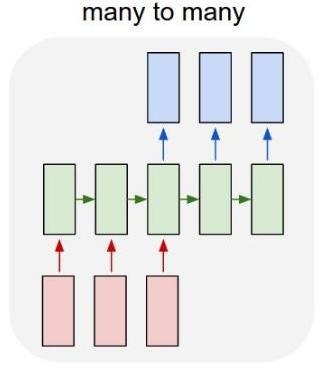
\includegraphics[keepaspectratio,
                     width=0.4\paperwidth]{many-to-many.jpg} \\
    Sentiment Classification & Machine Translation \\
     (sequence of words) $\to$ sentiment & (seq of words) $\to$ (seq of words)
  \end{tabular}
\end{frame}


\begin{frame}
  \begin{center}
    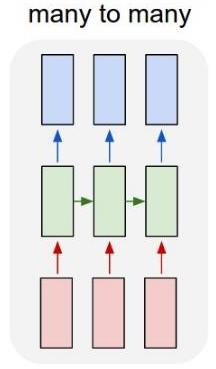
\includegraphics[keepaspectratio,
                     width=0.3\paperwidth]{many-to-many-2.jpg}

    Video Classification

    (on frame level)
  \end{center}
\end{frame}


\begin{frame}
  \frametitle{Последовательная обработка фиксированного входа}
  \begin{center}
    \animategraphics[loop,width=0.28\paperwidth,autoplay]{8}{house_read-}{0}{191}
  \end{center}

  \noindent\rule{8cm}{0.4pt}

  \href{https://arxiv.org/abs/1412.7755}{J. Ba, V. Mnih, K. Kavukcuoglu. Multiple Object Recognition with Visual Attention}
\end{frame}

\begin{frame}
  \frametitle{Последовательная генерация фиксированного выхода}
  \begin{center}
    \animategraphics[loop,width=0.5\paperwidth,autoplay]{8}{house_generate-}{0}{37}
  \end{center}

  \noindent\rule{8cm}{0.4pt}

  \href{https://arxiv.org/abs/1502.04623}{K. Gregor, I. Danihelka, A. Graves, D. J. Rezende, D. Wierstra. DRAW: A Recurrent Neural Network For Image Generation}
\end{frame}


\begin{frame}[t]
  \frametitle{Рекуррентная нейронная сеть (RNN)}
  \begin{center}
    \begin{picture}(150, 125)
      \multiput(0,0)(35, 0){6}{
        \put(-25, 45){\vector(1, 0){25}}
      }
      \multiput(0,0)(35, 0){5}{
        \put(5, 5){\vector(0, 1){25}}
        \put(5, 60){\vector(0, 1){25}}
      }
      \multiput(0,0)(35, 0){5}{
        \put(0, 0){
          \put(0, 30){\framebox(10, 30){}}
        }
      }
      \put(-2, 0){\makebox{$x_{t-2}$}}
      \put(33, 0){\makebox{$x_{t-1}$}}
      \put(71, 0){\makebox{$x_{t}$}}
      \put(103, 0){\makebox{$x_{t+1}$}}
      \put(138, 0){\makebox{$x_{t+2}$}}
      \put(70, 42){\makebox{$h_{t}$}}
      \put(-2, 89){\makebox{$y_{t-2}$}}
      \put(33, 89){\makebox{$y_{t-1}$}}
      \put(71, 89){\makebox{$y_{t}$}}
      \put(103, 89){\makebox{$y_{t+1}$}}
      \put(138, 89){\makebox{$y_{t+2}$}}
    \end{picture}
  \end{center}

\end{frame}


\begin{frame}[t]
  \frametitle{Рекуррентная нейронная сеть (RNN)}

  Обрабатываем последовательность векторов $x$ {\bf одной и той же} функцией с параметрами:

  $$ h_t = f_W(h_{t-1}, x_t)$$

  $f_W$ — функция, параметризованная $W$

  $x_t$ — очередной входной вектор

  $h_t$ — скрытое состояние
  \pause
  \begin{question}
  Какую функцию взять в качестве $f_W$?
  \end{question}
\end{frame}


\begin{frame}[t]
  \frametitle{Простейшая (vanilla) рекуррентная нейронная сеть}

  $$ h_t = f_W(h_{t-1}, x_t)$$

  В качестве функции $f_W$ задаём линейное преобразование с нелинейной «сигмоидой» по компонентам:

  \begin{align*}
    h_t &= \tanh ({\color{red}W_{hh}} h_{t-1} + {\color{red}W_{xh}} x_t) \\
    y_t &= {\color{red}W_{hy}} h_t
  \end{align*}
\end{frame}


\begin{frame}
  \frametitle{Пример модели на уровне символов}

   Весь словарь из четырёх букв: $[h, e, l, o]$

   \begin{center}
     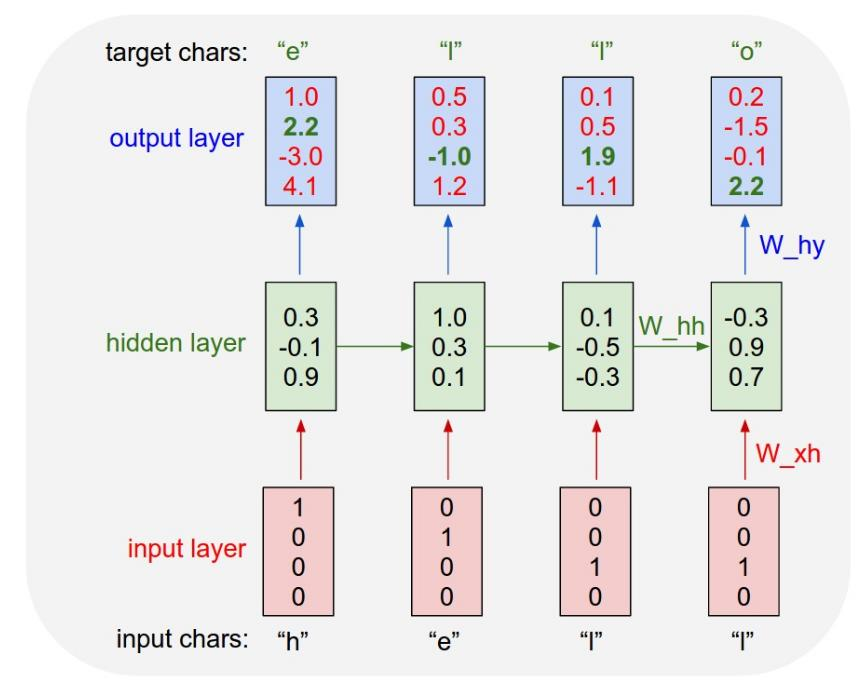
\includegraphics[keepaspectratio,
                      width=0.6\paperwidth]{rnn_char_level_example.jpg}
   \end{center}

   к значениям выходного слоя для получения функции потерь ещё применяется {\bf Softmax}

\end{frame}


\begin{frame}
  \frametitle{Демо}

  \href{https://gist.github.com/karpathy/d4dee566867f8291f086}{Реализация на \pyth{numpy} от Karpathy}

  \vspace{1cm}
  \href{https://github.com/spbu-math-cs/ml-course/blob/main/2022-spring-part-2/lectures/03_rnn/03_rnn_demo.ipynb}{Разбираемся с кодом!}
\end{frame}


\begin{frame}
  \frametitle{Как это работает?}

  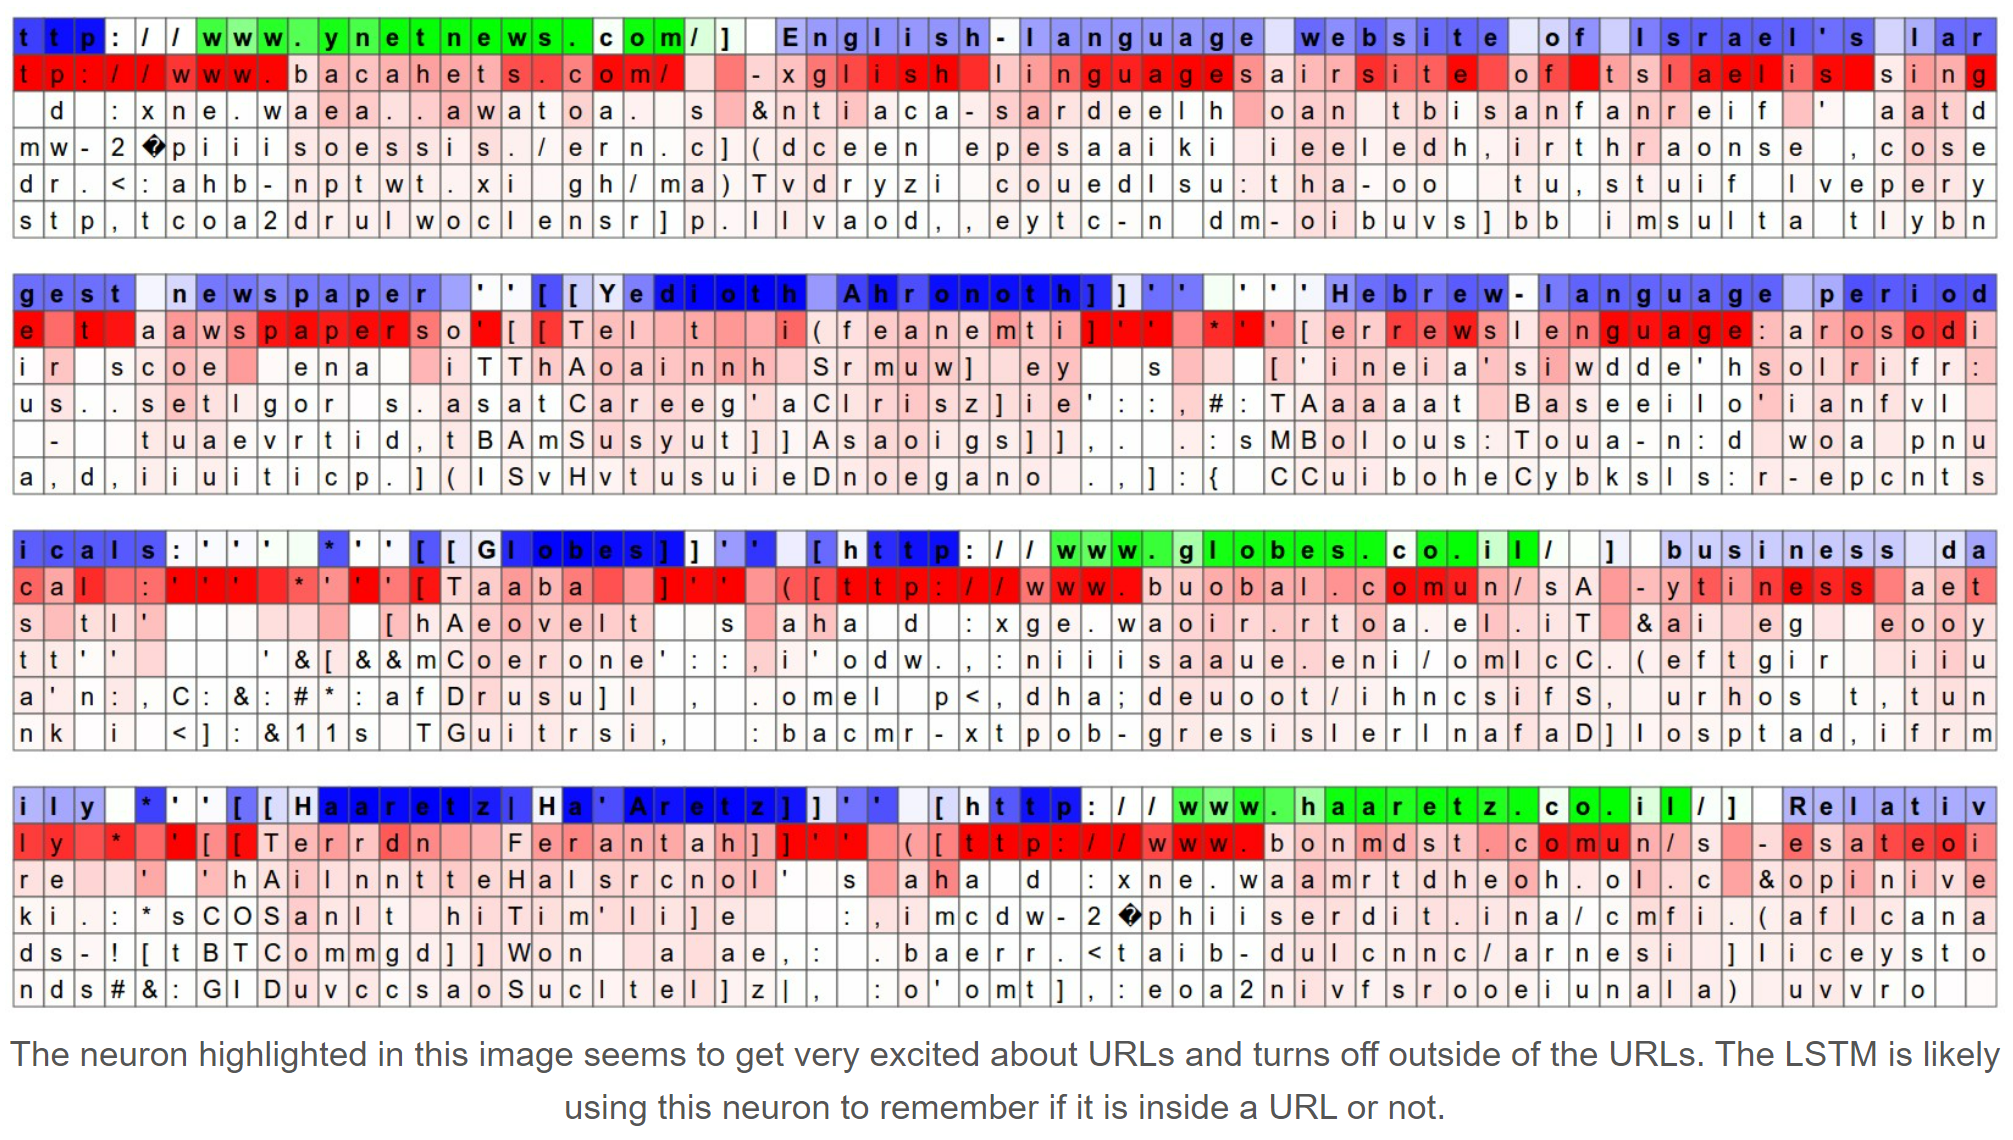
\includegraphics[keepaspectratio,
                   width=.85\paperwidth]{url_neuron.png}

\end{frame}


\begin{frame}
  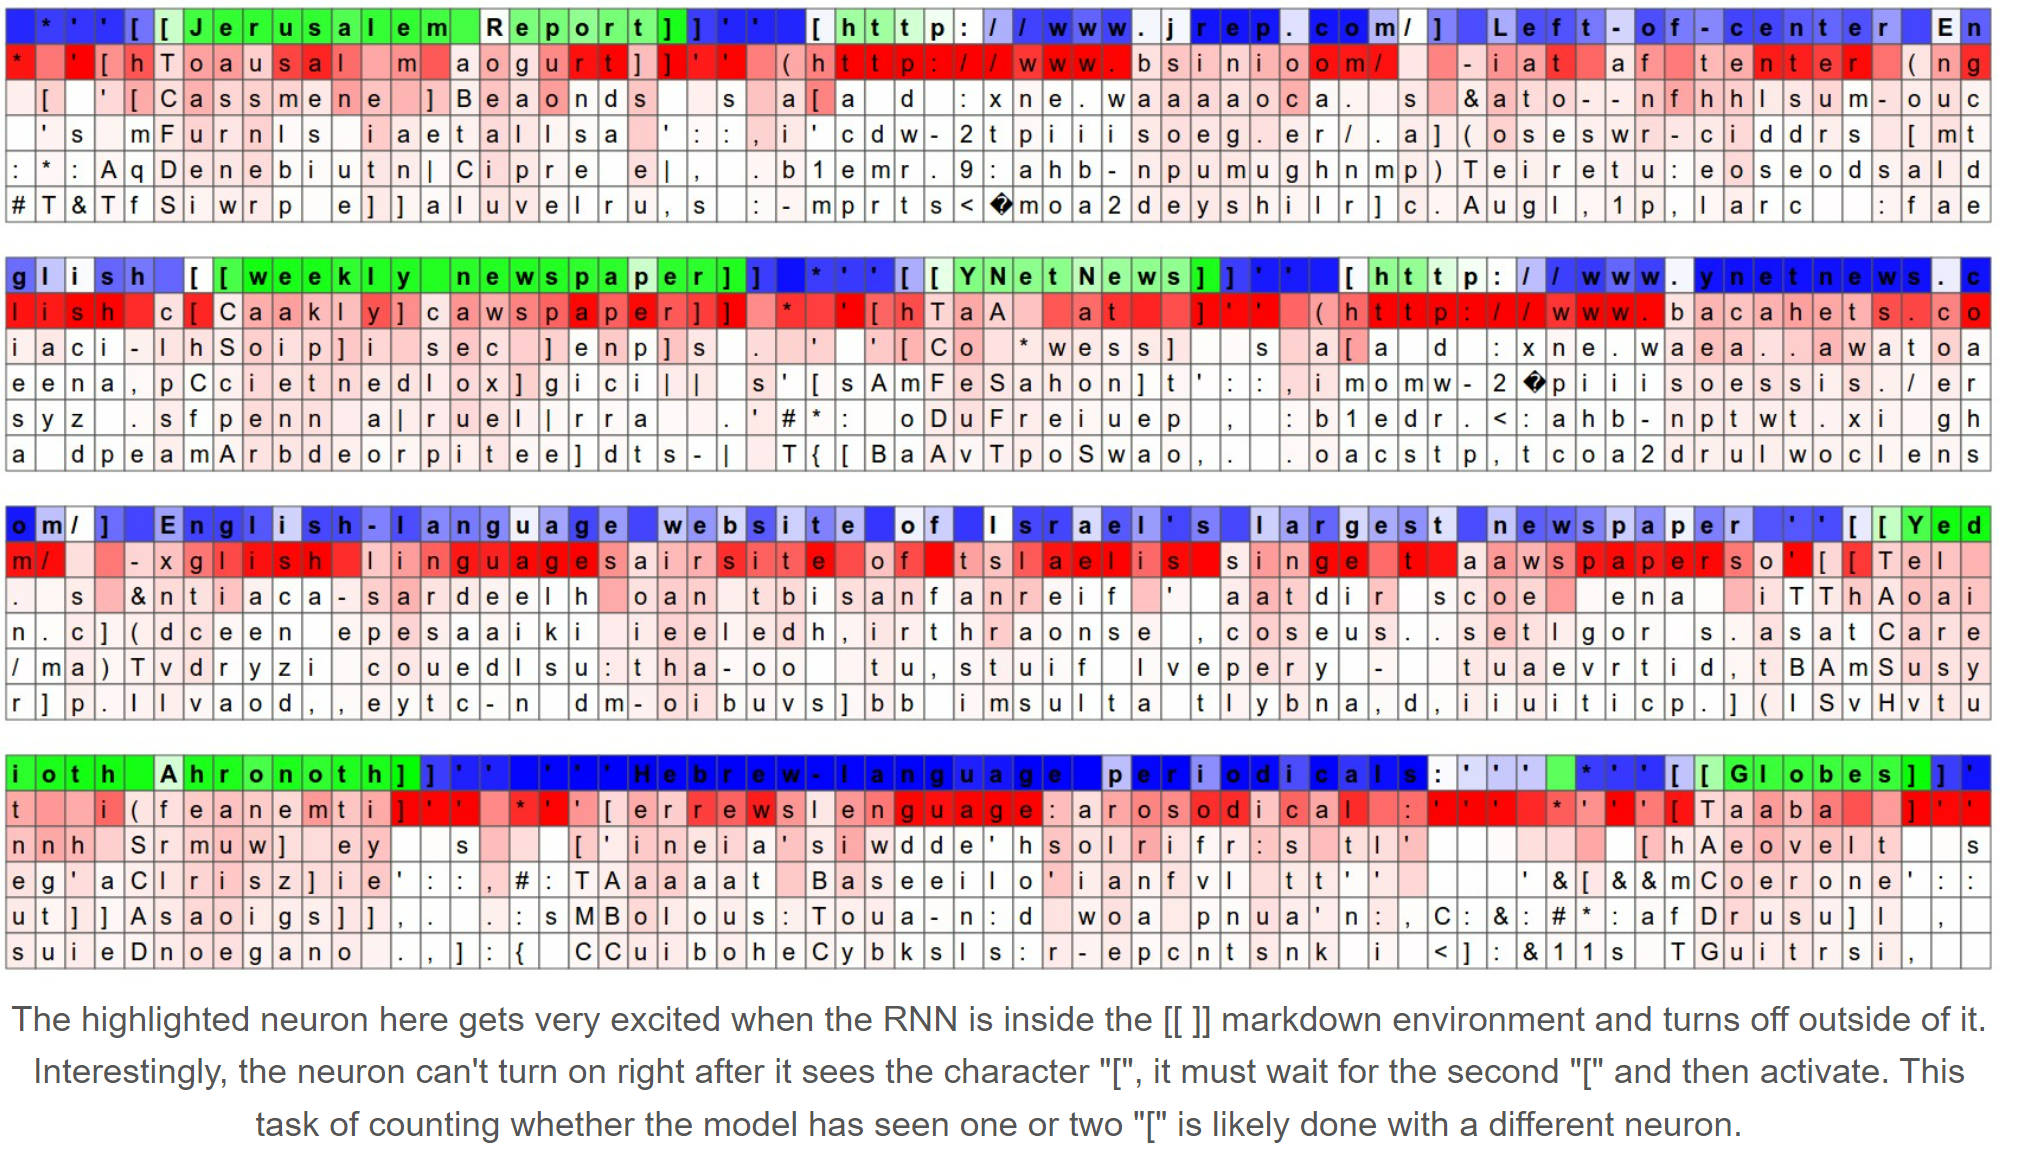
\includegraphics[keepaspectratio,
                   width=.85\paperwidth]{bracket_neuron.png}

\end{frame}


\begin{frame}
  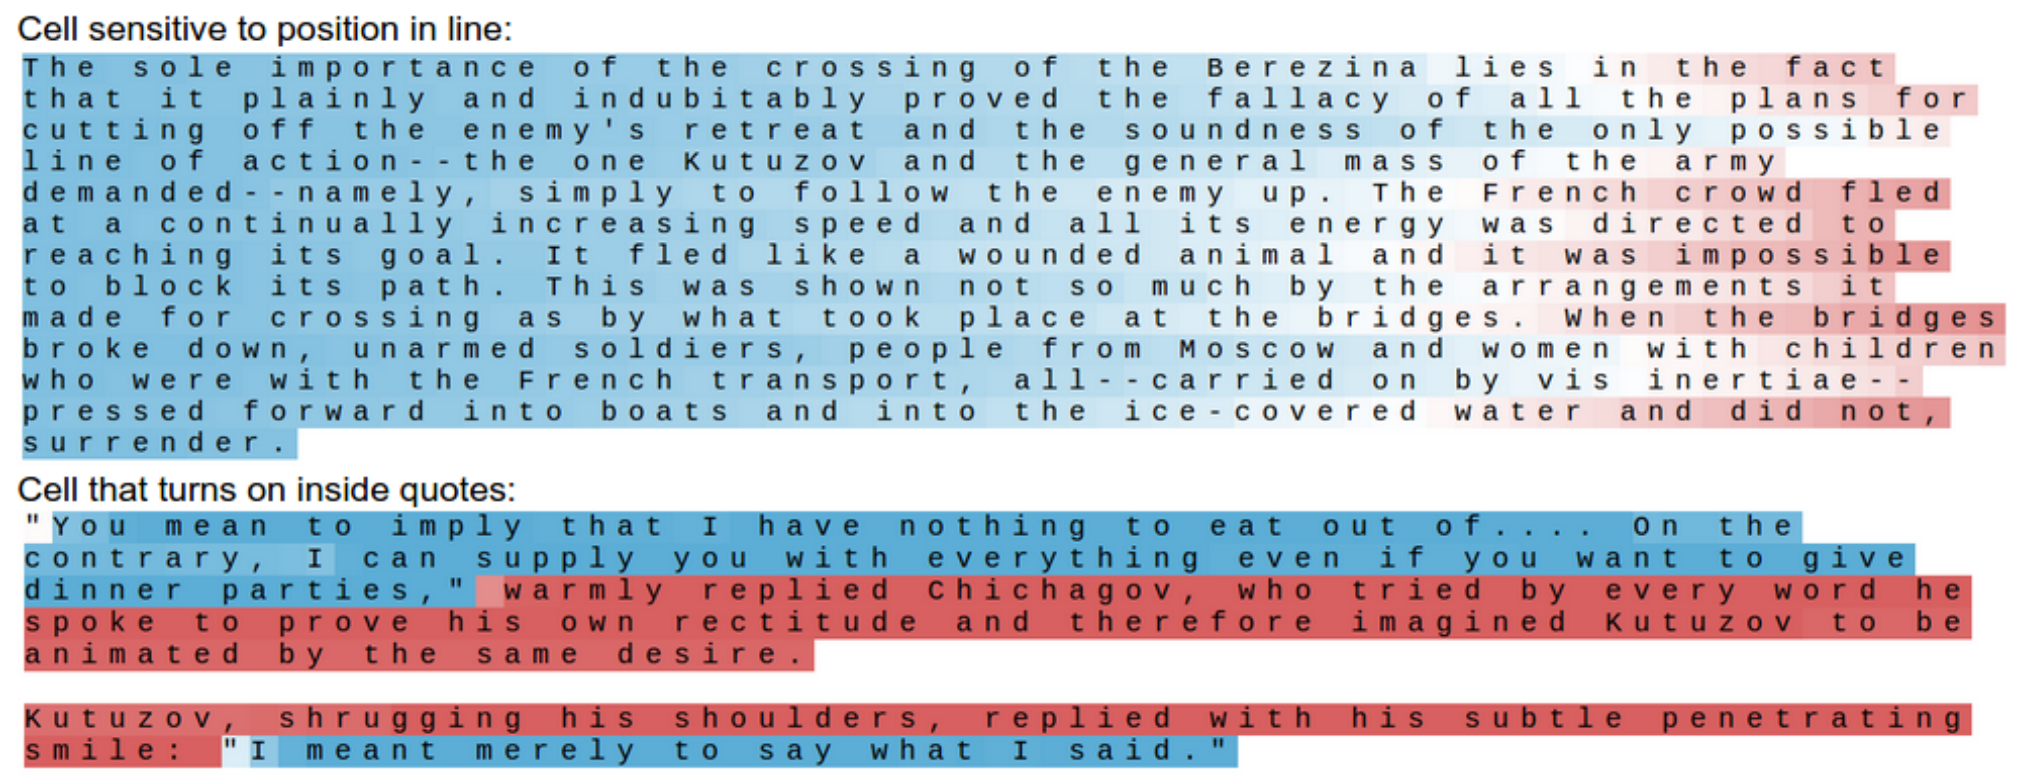
\includegraphics[keepaspectratio,
                   width=.85\paperwidth]{cell_endline.png}

\end{frame}


\begin{frame}
  \frametitle{Глубокие рекуррентные сети}
  \begin{columns}
      \begin{column}{.4\paperwidth}
        $\quad h_t^\ell = \tanh W^\ell \left(\begin{array}{c}
         h_t^{\ell-1} \\ h_{t-1}^{\ell}
        \end{array}\right)$

        $\quad h \in \mathbb{R}^n, \quad\quad W^\ell [n \times 2n]$
      \end{column}
      \begin{column}{.4\paperwidth}
        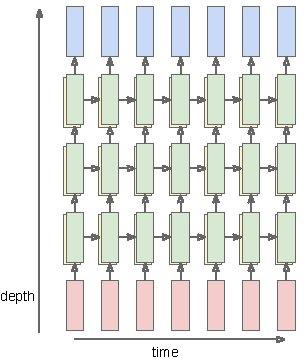
\includegraphics[keepaspectratio,
                         width=0.4\paperwidth]{rnn_depth.jpg}
      \end{column}
  \end{columns}
  \pause
  \begin{question}
  Какая главная проблема vanilla RNN?
  \end{question}
\end{frame}


\begin{frame}[t]
  \frametitle{Долгая кратковременная память (Long short-term memory, LSTM)}

  \begin{align*}
     &W^\ell [4n\times 2n] \\
    \left(\begin{array}{c}
    i \\ f \\ o \\ c_t^\prime
    \end{array}\right) &=
    \left(\begin{array}{c}
    \text{sigm} \\ \text{sigm} \\ \text{sigm} \\ \tanh
    \end{array}\right)
    W^\ell
    \left(\begin{array}{c}
    h_t^{\ell-1} \\ h_{t-1}^{\ell}
    \end{array}\right) \\
    &\begin{array}{l}
    c_t^\ell = f \odot c_{t-1}^\ell + i \odot c_t^\prime \\
    h_t^\ell = o \odot \tanh(c_t^\ell)
    \end{array}
  \end{align*}
  \center $\odot$ - покомпонентное произведение
\end{frame}


\begin{frame}
  \frametitle{Мотивация и схема LSTM}

  Сеть должна долго помнить контекст. Какой именно сеть выучивает сама.
  Для этого вводится вектор $c_t$ — вектор состояния сети в момент $t$.

  \vspace{1cm}
  \begin{tabular}{ll}
    $c_t^\prime = \tanh(W_{xc}x_t + W_{hc}h_{t-1} + b_{c^\prime})$ & candidate cell state \\
    $i_t = \sigma(W_{xi}x_t + W_{hi}h_{t-1} + b_{i})$ & input gate \\
    $f_t = \sigma(W_{xf}x_t + W_{hf}h_{t-1} + b_{f})$ & forget gate \\
    $o_t = \sigma(W_{xo}x_t + W_{ho}h_{t-1} + b_{o})$ & output gate \\
     & \\
    $c_t = f_t \odot c_{t-1} + i_t \odot c_t^\prime$ & cell state \\
    $h_t = o_t \odot \tanh(c_t)$ & block output
  \end{tabular}
\end{frame}

\begin{frame}
  \begin{tikzpicture}[
    % GLOBAL CFG
    font=\sf \scriptsize,
    >=LaTeX,
    % Styles
    cell/.style={% For the main box
        rectangle,
        rounded corners=5mm,
        draw,
        very thick,
        },
    operator/.style={%For operators like +  and  x
        circle,
        draw,
        inner sep=-0.5pt,
        minimum height =.2cm,
        },
    function/.style={%For functions
        ellipse,
        draw,
        inner sep=1pt
        },
    ct/.style={% For external inputs and outputs
        circle,
        draw,
        line width = .75pt,
        minimum width=1cm,
        inner sep=1pt,
        },
    gt/.style={% For internal inputs
        rectangle,
        draw,
        minimum width=4mm,
        minimum height=3mm,
        inner sep=1pt
        },
    mylabel/.style={% something new that I have learned
        font=\scriptsize\sffamily
        },
    ArrowC1/.style={% Arrows with rounded corners
        rounded corners=.25cm,
        thick,
        },
    ArrowC2/.style={% Arrows with big rounded corners
        rounded corners=.5cm,
        thick,
        },
    ]

    %Start drawing the thing...
    % Draw the cell:
    \node [cell, minimum height =4cm, minimum width=6cm] at (0,0){} ;

    % Draw inputs named ibox#
    \node [gt] (ibox1) at (-2,-0.75) {$\sigma$};
    \node [gt] (ibox2) at (-1.5,-0.75) {$\sigma$};
    \node [gt, minimum width=1cm] (ibox3) at (-0.5,-0.75) {Tanh};
    \node [gt] (ibox4) at (0.5,-0.75) {$\sigma$};

   % Draw opérators   named mux# , add# and func#
    \node [operator] (mux1) at (-2,1.5) {$\times$};
    \node [operator] (add1) at (-0.5,1.5) {+};
    \node [operator] (mux2) at (-0.5,0) {$\times$};
    \node [operator] (mux3) at (1.5,0) {$\times$};
    \node [function] (func1) at (1.5,0.75) {Tanh};

    % Draw External inputs? named as basis c,h,x
    \node[ct, label={[mylabel]Cell}] (c) at (-4,1.5) {\empt{c}{t-1}};
    \node[ct, label={[mylabel]Hidden}] (h) at (-4,-1.5) {\empt{h}{t-1}};
    \node[ct, label={[mylabel]left:Input}] (x) at (-2.5,-3) {\empt{x}{t}};

    % Draw External outputs? named as basis c2,h2,x2
    \node[ct, label={[mylabel] }] (c2) at (4,1.5) {\empt{c}{t}};
    \node[ct, label={[mylabel] }] (h2) at (4,-1.5) {\empt{h}{t}};
    \node[ct, label={[mylabel]left: }] (x2) at (2.5,3) {\empt{h}{t}};

   % Start connecting all.
    %Intersections and displacements are used.
    % Drawing arrows
    \draw [ArrowC1] (c) -- (mux1) -- (add1) -- (c2);

    % Inputs
    \draw [ArrowC2] (h) -| (ibox4);
    \draw [ArrowC1] (h -| ibox1)++(-0.5,0) -| (ibox1);
    \draw [ArrowC1] (h -| ibox2)++(-0.5,0) -| (ibox2);
    \draw [ArrowC1] (h -| ibox3)++(-0.5,0) -| (ibox3);
    \draw [ArrowC1] (x) -- (x |- h)-| (ibox3);

    % Internal
    \draw [->, ArrowC2] (ibox1) -- (mux1);
    \node at ($(ibox1)!0.3!(mux1)+(-0.2,0)$) {$f_t$};
    \draw [->, ArrowC2] (ibox2) |- (mux2);
    \node at ($(ibox2)!0.4!(mux2)+(-0.2,0)$) {$i_t$};
    \draw [->, ArrowC2] (ibox3) -- (mux2);
    \draw [->, ArrowC2] (ibox4) |- (mux3);
    \node at ($(ibox4)!0.4!(mux3)+(-0.2,0)$) {$o_t$};
    \draw [->, ArrowC2] (mux2) -- (add1);
    \draw [->, ArrowC1] (add1 -| func1)++(-0.5,0) -| (func1);
    \draw [->, ArrowC2] (func1) -- (mux3);

    %Outputs
    \draw [-, ArrowC2] (mux3) |- (h2);
    \draw (c2 -| x2) ++(0,-0.1) coordinate (i1);
    \draw [-, ArrowC2] (h2 -| x2)++(-0.5,0) -| (i1);
    \draw [-, ArrowC2] (i1)++(0,0.2) -- (x2);
  \end{tikzpicture}
\end{frame}

\begin{frame}
  \frametitle{LSTM: forget gate}
    $ f_t = \sigma(W_{xf}x_t + W_{hf}h_{t-1} + b_{f}) $

  \vspace{1cm}
  Пример: удаление пола действующего лица при генерации текста
\end{frame}


\begin{frame}
  \frametitle{LSTM: input/candidate gates}
  \begin{tabular}{ll}
    $ c_t^\prime = \tanh(W_{xc}x_t + W_{hc}h_{t-1} + b_{c^\prime})$ & candidate cell state \\
    $ i_t = \sigma(W_{xi}x_t + W_{hi}h_{t-1} + b_{i})$ &  input gate
  \end{tabular}

  \vspace{1cm}
  Пример: добавление пола действующего лица при генерации текста
\end{frame}


\begin{frame}
  \frametitle{LSTM: обновление состояния ячейки памяти}
    $ c_t = f_t \odot c_{t-1} + i_t \odot c_t^\prime \quad$ (cell state)

  \vspace{1cm}
  Новое состояние $c_t$ получается суммой предыдущего состояния $c_{t-1}$ с фильтром $f_t$ и вектора значений-кандидатов $c_t^\prime$ с фильтром $i_t$
\end{frame}


\begin{frame}
  \frametitle{LSTM: генерация выхода}
  \begin{tabular}{ll}
    $ o_t = \sigma(W_{xo}x_t + W_{ho}h_{t-1} + b_{o})$ & output gate \\
    $ h_t = o_t \odot \tanh(c_t)$ & block output
  \end{tabular}
\end{frame}


\begin{frame}
  \frametitle{GRU: Gated Recurrent Unit}
  \begin{align*}
      u_t &= \sigma(W_{xu}x_t + W_{hu}h_{t-1} + b_{u}) \\
      r_t &= \sigma(W_{xr}x_t + W_{hr}h_{t-1} + b_{r}) \\
      h_t^\prime &= \tanh(W_{xh^\prime}x_t + W_{hh^\prime}(r_t\odot h_{t-1})) \\
      h_t &= (1-u_t) \odot h_t^\prime + u_t \odot h_{t-1}
  \end{align*}

  Используется только $h_t$, вектор $c_t$ не вводится.

  Фильтр обновления (update gate) вместо входного и забывающего.

  Фильтр перезагрузки (reset gate) определяет, какую часть памяти перенести дальше с предыдущего шага.
\end{frame}

\begin{frame}
  \frametitle{Резюме}
  \begin{itemize}
    \item Рекуррентные нейронные сети — простой, мощный и гибкий подход решения различных задач машинного обучения
    \item Vanilla RNN просты, но всё-таки недостаточно хороши
    \item Поэтому нужно использовать LSTM или GRU
    \item Зануление градиентов предотвращает LSTM
    \item От <<взрыва градиентов>> помогает clipping
    \item Необходимо более глубокое понимание, как теоретическое, так и практическое — много открытых вопросов
  \end{itemize}
  \pause
  Что ещё можно посмотреть?
  \begin{itemize}
    \item \href{https://www.youtube.com/watch?v=iX5V1WpxxkY}{Лекция 10} курса <<CS231n>> Andrej Karpathy в Стенфорде
    \item Как \href{http://karpathy.github.io/2019/04/25/recipe/}{тренировать нейросети}?
    \item \href{https://github.com/yandexdataschool/Practical_DL/tree/fall21/week06_rnn}{Аналогичное занятие} курса Школы анализа данных
  \end{itemize}
\end{frame}

\end{document}
